\documentclass[journal,twoside,web]{ieeecolor}
\pdfminorversion=4
\usepackage{generic}


\usepackage{cite}
\usepackage{amsmath,amssymb,amsfonts}
\usepackage{graphicx}
\usepackage{algorithm}
\usepackage[hidelinks]{hyperref}
\usepackage{textcomp}

\usepackage[utf8]{inputenc} % allow utf-8 input
\usepackage[T1]{fontenc}    % use 8-bit T1 fonts
\usepackage{algpseudocode}
\usepackage{multirow}
\usepackage{url}
\usepackage{xcolor}
\usepackage{optidef}
\usepackage{arydshln}
\usepackage{balance}
\usepackage{tikz}
\usepackage{circuitikz}
\usetikzlibrary{arrows.meta}
\tikzstyle{block} = [draw, rectangle, 
    minimum height=3em, minimum width=3em]
\tikzstyle{sum} = [draw, circle, node distance=1cm]
\tikzstyle{input} = [coordinate]
\tikzstyle{output} = [coordinate]
\tikzstyle{pinstyle} = [pin edge={to-,thin,black}]

\graphicspath{{./figures/}}

\usepackage{bbm}

\newtheorem{theorem}{Theorem}
\newtheorem{lemma}[theorem]{Lemma}
\newtheorem{corollary}{Corollary}[theorem]
\newtheorem{remark}{Remark}
\newtheorem{definition}{Definition}
\newtheorem{exmp}{Example}


%
\newcommand{\dsp}{\displaystyle}
\newcommand{\BBM}{\begin{bmatrix}}
\newcommand{\EBM}{\end{bmatrix}}
\newcommand{\BEQ}{\begin{equation}}
\newcommand{\EEQ}{\end{equation}}
\newcommand{\BIT}{\begin{itemize}}
\newcommand{\EIT}{\end{itemize}}
\newcommand{\cf}{{\it cf.}}
\newcommand{\eg}{{\it e.g.}}
\newcommand{\ie}{{\it i.e.}}
\newcommand{\st}{\mbox{subject to}}
\newcommand{\ones}{\mathbbm{1}}
\newcommand{\reals}{\mathbb{R}}
\newcommand{\ereals}{\bar{\reals}}
\newcommand{\pereals}{(-\infty,+\infty]}
\newcommand{\naturals}{\mathbb{N}}
\newcommand{\symm}{\mathbb{S}}
\newcommand{\quadcone}{\mathbb{Q}}
\newcommand{\expcone}{K_{\exp}}
\newcommand{\complex}{\mathbb{C}}
\newcommand{\integers}{\mathbb{Z}}
\newcommand{\psimplex}{\Delta}
\newcommand{\eqbydef}{\mathrel{\stackrel{\Delta}{=}}}
\newcommand{\im}{\mathrm{i}}
\newcommand{\minimize}{\mbox{minimize}}
\newcommand{\maximize}{\mbox{maximize}}
\newcommand{\Range}{\mathcal{R}}
\newcommand{\nullspace}{\mathcal{N}}
\newcommand{\feasset}{\mathcal{F}}
\newcommand{\probdom}{\mathcal{D}}

\newcommand{\argit}[2]{#1_{#2}}
\newcommand{\xit}[1]{\argit{x}{#1}}
\newcommand{\majf}{\bar f}
\newcommand{\maj}[2]{\majf(#1\,\vert\,#2)}
\newcommand{\indicator}[1]{I_{#1}}


\DeclareMathOperator{\Span}{span}
\DeclareMathOperator{\nullity}{nullity}
\DeclareMathOperator{\rank}{rank}
\DeclareMathOperator{\Tr}{tr}
\DeclareMathOperator{\diag}{diag}
\DeclareMathOperator{\blkdiag}{blkdiag}
\DeclareMathOperator{\vect}{vec}
\DeclareMathOperator{\svect}{svec}
\DeclareMathOperator{\dom}{dom}
\DeclareMathOperator{\conv}{conv}
\DeclareMathOperator{\relint}{relint}
\DeclareMathOperator{\interior}{int}
\DeclareMathOperator{\aff}{aff}
\DeclareMathOperator{\cone}{cone}
\DeclareMathOperator{\epi}{epi}
\DeclareMathOperator{\cl}{cl}
\DeclareMathOperator*{\argmin}{argmin}
\DeclareMathOperator*{\argmax}{argmax}
\DeclareMathOperator{\sgn}{sgn}
\DeclareMathOperator{\prox}{prox}
\DeclareMathOperator{\nnz}{nnz}

\DeclareMathOperator{\sqr}{sqr}
\DeclareMathOperator{\adj}{adj}
\DeclareMathOperator{\bdiag}{bdiag}

\DeclareMathOperator{\Expect}{\mathbb{E}}
\DeclareMathOperator{\Var}{Var}

\newcommand{\E}[2][]{\Expect_{#1}\!\left[\,#2\,\right]}   % Expectation with argument
\newcommand{\CE}[2]{\E{#1 \,\middle|\, #2}}                              % Conditional expectation

\DeclareMathOperator{\Probability}{\mathbb{P}}
\newcommand{\Prob}[2][]{\Probability_{#1}\!\left[\,#2\,\right]}     % Probability with argument
\newcommand{\CProb}[2]{\Prob{#1 \,\middle|\, #2}}                       % Conditional probability

\newcommand{\tnabla}{\widetilde{\nabla}}


\newcommand{\mfile}[1]{\txtmint{#1}}
\newcommand{\mfilelabel}[2]{\txtmint{#1}}


\AtBeginDocument{%
\setlength{\abovedisplayskip}{5pt plus 2pt minus 1pt}%
\setlength{\belowdisplayskip}{5pt plus 2pt minus 1pt}%
\setlength{\abovedisplayshortskip}{0pt plus 2pt}%
\setlength{\belowdisplayshortskip}{5pt plus 2pt minus 1pt}%
}
%
\def\BibTeX{{\rm B\kern-.05em{\sc i\kern-.025em b}\kern-.08em
    T\kern-.1667em\lower.7ex\hbox{E}\kern-.125emX}}
\markboth{IEEE TRANSACTIONS ON AUTOMATIC CONTROL}
{Hansson \MakeLowercase{\textit{et al.}}: Informativity and Identifiability for Identification of Networks of Dynamical Systems}

\begin{document}
%
\title{Informativity and Identifiability for Identification of Networks of Dynamical Systems}
\author{Anders Hansson, \IEEEmembership{Senior Member, IEEE}, João Victor Galvão da Mata, and Martin S.~Andersen
\thanks{This work was supported by ELLIIT, and by the Novo Nordisk Foundation under grant number NNF20OC0061894.}
\thanks{Anders Hansson is with the Department of Electrical Engineering, Linköping University (e-mail: anders.g.hansson@liu.se).}
\thanks{João Victor Galvão da Mata and Martin S.~Andersen are with the Department of Applied Mathematics and Computer Science, Technical University of Denmark (e-mail: jogal@dtu.dk; mskan@dtu.dk).}}
%
\maketitle
%
\begin{abstract}
%
We study informativity and network identifiability for dynamic networks
with unknown input and measurement transfer functions, constrained entries,
and repeated open-loop transfer functions. Positive definiteness of the external-signal
spectrum and full generic row rank of the transfer function matrix from external signals to the predictor
inputs give a sufficient condition for generic informativity. We determine
this rank by disjoint paths for independent entries and by a Gröbner basis
test for constrained entries. The dimension of the generic fiber of the
map from open-loop to closed-loop transfer functions determines whether finitely many networks
are compatible with the same closed-loop transfer function. A repeated-entry
example has two
admissible networks in a generic fiber, an ambiguity that generic Jacobian
rank alone does not count.
%
\end{abstract}
%
\begin{IEEEkeywords}
System Identification, Networks, Dynamical Systems, Informativity, Generic local network identifiability.
\end{IEEEkeywords}
%
\section{Introduction}
%
\IEEEPARstart{S}{ystem} identification for networks of dynamical systems is an active research 
field with a 
long history. Some early references 
are \cite{VANDENHOF19931523,VANDENHOF20132994,hen+gev+baz19}. Some of the work has been focusing on identifying
the full network, e.g. \cite{FONKEN2022110295,hen+gev+baz19,WEERTS2018256}, while other work has been focusing on identifying parts of the network,
or {\it subnetworks}, e.g.
\cite{VANDENHOF20132994,Dankers_predictor_input,Materassi2019SignalSF,7402842,Linder03042017,9247487,9661422}.
The latter is an example of system 
identification under feedback, a topic that also has a long history, see e.g. \cite{FORSSELL19991215}.

Prediction error methods use a predictor to estimate an output from measured
signals. Their analysis raises two distinct questions. Informativity asks whether
the data determine the predictor within a candidate model class. Network
identifiability asks whether the resulting closed-loop transfer functions
determine the open-loop transfer functions in the network. The latter question differs
from identifiability of a particular numerical parametrization. We study
generic properties of the specified model class: properties that can fail
only on a proper algebraic subset of its admissible networks. In particular,
generic local network identifiability in the algebraic sense allows finitely
many networks to share the same closed-loop transfer function.
This is related to structural identifiability, which asks whether the
parameters of a specified dynamical model can be recovered from its
input-output behavior; Ljung and Glad study global identifiability for
general nonlinear model structures using differential algebra
\cite{LjungGlad1994}. Our identifiability target is instead the unknown
open-loop transfer functions of a specified network structure, and our
generic local criterion permits finite ambiguity.

Prior work addresses partial node measurement
\cite{hen+gev+baz19,9303890,SHI2022110093} and data informativity
\cite{VANDENHOF20132994,BOMBOIS2023110742}. The novel aspects of this
paper relative to these and the cited rank and identifiability results are:
\begin{itemize}
\setlength{\itemsep}{0pt}\setlength{\parsep}{0pt}\setlength{\topsep}{2pt}
\item The novel model scope is the joint treatment of unknown input and
measurement transfer functions, direct input-to-output paths, and repeated
or constrained transfer functions. The network models in
\cite{hen+gev+baz19,9303890} use fixed input and measurement selections.
\item The novel aspect of the rank analysis is its application to this
model: disjoint paths include direct input-to-output paths, while
polynomial elimination handles known relations among entries. The
path-rank principle \cite{wou91} and spectral informativity implication
\cite{Ljung1999} are established results.
\item The novel identifiability contribution is applying the standard
algebraic dimension criterion \cite{cox+lit+she92} to the map from open-loop
to closed-loop transfer functions for this network class, including repeated and constrained
entries, and solving the resulting equations to expose finite ambiguity.
Example 3 demonstrates this with two compatible networks, which generic
Jacobian rank alone does not count.
\end{itemize}
%
\section{Model of Network}
%
We consider a linear dynamic network model defined by 
%
\BEQ\label{eqn:PMD-model}
\begin{aligned}
P(q)w_k&=Q(q)u_k\\
z_k&=R(q)w_k+S(q)u_k
\end{aligned}
\EEQ
%
where $(P,Q,R,S)$ are rational transfer function matrices
in the forward shift operator $q$. The dimensions of these transfer function matrices are $n\times n$, 
$n\times m$, $p\times n$, and $p\times m$, respectively. This also defines the dimensions of all the 
signals, where $u_k$ is referred to as the input signal, $z_k$ as the output signal, and $w_k$ as the node signal.
The familiar model $w_k=G(q)w_k+B(q)u_k$, $z_k=C(q)w_k$, where $G$
contains node-to-node transfer functions, $B$ input-to-node transfer functions, and $C$
node-to-output transfer functions, is obtained with
$P=I-G$, $Q=B$, $R=C$, and $S=0$. Thus $P$ describes internal connections,
$Q$ describes how inputs enter the nodes, $R$ describes how nodes are measured,
and $S$ describes paths from inputs to outputs that bypass the nodes.
The model allows the input-to-node transfer functions in $Q$ and the
node-to-output transfer functions in $R$ to be unknown. It also allows
direct input-to-output paths through $S$ and known relations among entries
of $P,Q,R,S$. The form $Pw=Qu$ retains the coefficients of the original
node equations when
normalization would introduce shared factors into the input and connection
transfer functions. Filtered or combined sensor readings give $R$, while
direct input effects on measured outputs give $S$.
For example, physical networks with local node dynamics and diffusive
couplings can be written $D(q)w_k=K(q)w_k+B(q)u_k$, where diagonal $D$ contains
the local dynamics and $K$ the couplings \cite{KivitsVanDenHof2019}.
Here $P=D-K$ retains these physical coefficients and $Q=B$ retains the
separate input matrix. If $D$ is invertible, normalization gives
$G=D^{-1}K$ and an input transfer function matrix $D^{-1}B$, but these entries then share
unknown factors and relations inherited from $D$.
The constrained-entry tests below retain these relations.
The notation also accommodates a discrete-time descriptor model
$Ew_{k+1}=Aw_k+Bu_k$, $z_k=Cw_k+Du_k$, where $E,A,B,C,D$ are real
matrices and $\det(qE-A)$ is not identically zero. It has $P(q)=qE-A$,
$Q=B$, $R=C$, and $S=D$. When $E$ is singular, this representation
retains the algebraic equations alongside the state dynamics.
Prescribed zero patterns and known coefficients in these matrices
specify a constrained model class. Its unknown matrix entries are real
constants, and the coefficients of $P(q)=qE-A$ retain this structure.
We assume that the structural zero pattern and any known entries or relations
among unknown entries of $(P,Q,R,S)$ are specified. The task is to determine
these entries for the given model class and zero pattern.
Structurally free entries may take the value zero at exceptional realizations.
We assume that $P$ is generically invertible: $\det P$, viewed as a rational
expression in its free entries, is not identically zero. A generic choice
of these entries then gives an invertible rational matrix $P$. We call
a realization {\it well-posed} when its $P$ is invertible and apply formulas
involving $P^{-1}$ only to such realizations. When evaluating a transfer
function, we use $\lambda\in\mathbb C$ as its complex argument, for example
$P(\lambda)$. For a well-posed realization, $P(\lambda)$ is invertible at
all but finitely many $\lambda$ where its entries are defined. Stability is
assumed separately when needed. Generic invertibility is checked from $P$
in each example.
Let $\theta$ denote the unknown parameters and $\theta_0$ their values in the
true network. When needed, we write $P(q;\theta)$ and $y_k(\theta)$ to show
parameter dependence. We otherwise omit the arguments $q$ and $\theta$.
%
\section{Innovation form and Predictor}\label{sec:innovation}
%
We partition $u_k$ into a measured input $r_k$ and an unmeasured noise input $e_k$.
We write $u_k=(r_k,e_k)$, where $r_k$ has $m_r$ components and $e_k$
has $m_e$ components. We also partition $Q(q)$ and $S(q)$ conformably as 
%
$$Q(q)=\BBM Q_r(q)&Q_e(q)\EBM,\quad S(q)=\BBM S_r(q)&S_e(q)\EBM.$$
We assume that the signals available to the predictor form
$z_k=(y_k,r_k)$. Here $y_k$ has $p_y$ components, and
$r_k$ has $m_r$ components, so $p=p_y+m_r$.
The measured outputs $y_k$ and inputs $r_k$ specify which predictor is
considered. For a subnetwork, measured node signals at its boundary can
also serve as measured inputs to that subnetwork.
We conformally write
%
\begin{align*}\BBM R(q)&S(q)\EBM&=\BBM R(q)&S_r(q)&S_e(q)\EBM\\&=
\BBM R_y(q)&S_{yr}(q)&S_{ye}(q)\\0&I&0\EBM
\end{align*}
%
for appropriately defined transfer function matrices. The resulting
closed-loop relation from $u_k$ to $y_k$ is
%
\BEQ
y_k=G_c(q)r_k+H_c(q)e_k\label{eqn:closed}
\EEQ
%
where
%
\BEQ\label{eqn:closed-tf}
\begin{aligned}
\BBM G_c(q)&H_c(q)\EBM&=R_y(q)P(q)^{-1}\BBM Q_r(q)&Q_e(q)\EBM\\&\quad+
\BBM S_{yr}(q)&S_{ye}(q)\EBM.
\end{aligned}
\EEQ
%
Assume that the measured output has an innovation representation
%
\begin{align}
\hat y_k&=G_c(q) r_k+G_o(q)\epsilon_k\label{eqn:innovation}\\
y_k&=\hat y_k+\epsilon_k\label{eqn:error}
\end{align}
%
where $G_o(q)$ is a transfer function matrix and the innovations
$\epsilon_k$ are independent, identically distributed zero-mean random
vectors. Such a representation can require solving an algebraic Riccati
equation \cite{hansson2025identifiabilitymaximumlikelihoodestimation}.
Only its existence is used here.

From the above equations we realize that we may write
%
\BEQ
\hat y_k= W(q)z_k\label{eqn:pred}
\EEQ
%
where 
%
$$W(q)=\BBM W_y(q)&W_r(q)\EBM =(I+G_o(q))^{-1}\BBM G_o(q)&G_c(q)\EBM.$$ 
%
We assume that this predictor for $y_k$ is stable, meaning that all poles
of $W(q)$ lie strictly inside the unit circle; this is checked in each
example. Solving the displayed relation for $G_c$ gives
%
\BEQ\label{eqn:predtogc}
 G_c(q)=(I- W_y(q))^{-1} W_r(q).
\EEQ
%
Thus the predictor for the selected signals determines the corresponding
closed-loop transfer function $G_c$. The selection therefore specifies both
the predictor and the transfer function to identify.
When $R_y=I$, all node signals are measured. When its rows select individual
node signals, only those nodes are measured. The model also permits a
measurement equation with unknown measurement transfer functions, as in Example~3.
The input matrices $Q_r$ and $Q_e$ may likewise contain unknown input transfer
functions rather than fixed input selections.
%
\section{Informativity}
%
Throughout, ``almost all frequencies'' means outside a set of Lebesgue
measure zero on $[-\pi,\pi]$.
We investigate when the predictor can be determined from the measured signals.
Predictor uniqueness is the data requirement for prediction-error estimation;
recovering open-loop transfer functions from that predictor is a separate question.
We adapt the prediction-error definition of data informativity
in \cite{BOMBOIS2023110742}:
%
\begin{definition}
The signal $z_k$ is said to be {\it informative enough} if for any two parameters 
$\theta_1$ and $\theta_2$ such that the closed loop system is stable, it holds that 
%
\BEQ\label{eqn:informative}
\E{\left(\hat y_{k}(\theta_1)-\hat y_{k}(\theta_2)\right)
\left(\hat y_{k}(\theta_1)-\hat y_{k}(\theta_2)\right)^T}=0
\EEQ
%
implies that $ W\left(e^{i\omega};\theta_1\right)= W\left(e^{i\omega};\theta_2\right)$ for almost  
all $\omega$. 
\end{definition}
%
It holds that 
%
$$\hat y_k(\theta_1)
-\hat y_k(\theta_2)=\Delta W(q)z_k$$
%
where $\Delta W(q)= W(q;\theta_1)- W(q;\theta_2)$. 
From Parseval's formula, it follows that 
\eqref{eqn:informative} is equivalent to 
%
$$\Delta  W\left(e^{i\omega}\right)\Phi_z(\omega)
\Delta  W\left(e^{-i\omega}\right)^T=0$$
%
for almost all $\omega$, where $\Phi_z$ is the spectrum of $z_k$. Hence, a sufficient condition for the 
above equality to imply that $ W\left(e^{i\omega};\theta_1\right)= W\left(e^{i\omega};\theta_2\right)$ for almost  
all $\omega$, is that $\Phi_z(\omega)$ is positive definite for almost all 
$\omega$.

The closed-loop transfer function from $u_k=(r_k,e_k)$ to $z_k$ is
%
$$\Pi(q)=R(q)P(q)^{-1}Q(q)+S(q)$$
%
If the spectrum of $u_k$ is positive definite and
$\Pi\left(e^{i\omega};\theta_0\right)$ has full row rank for almost all
$\omega$, then the spectrum of $z_k$ is positive definite.
Positive definiteness of the predictor-input spectrum is a standard sufficient
condition for informativity \cite{Ljung1999}; related network-specific
excitation conditions are studied in \cite{5325719,BOMBOIS2023110742}.
Here $\Pi$ describes how the external
signals reach the selected predictor inputs.
The full-row-rank condition depends on the true network at $\theta_0$.
To obtain a condition for generic true networks, let
%
\BEQ
M(q)=\BBM P(q)&Q(q)\\-R(q)&S(q)\EBM.
\EEQ
%
As in \cite{BOMBOIS2023110742}, we investigate the {\it generic} rank
%
$$\rank_{g} \Pi=\max_{M\text{ in the model class}}\rank\Pi.$$
%
The rank is taken over the field of rational transfer functions. For the
free-entry results below, we treat the free entries of $M$ as indeterminates
(formal variables) over $\mathbb C(\lambda)$, the field of rational functions
in $\lambda$. These variables are algebraically independent, meaning that
they satisfy no nonzero polynomial relation over this field. Constraints
are treated separately.
For algebraically generic admissible assignments of rational transfer functions
to these indeterminates, the rank of $\Pi$ over $\mathbb C(\lambda)$ equals
$\rank_g\Pi$. Since its minors are
rational functions of $\lambda$, this rank also holds at all but finitely
many $\lambda$ where $\Pi$ is defined. This gives a sufficient condition
for informativity at algebraically generic true networks.
%
\begin{theorem}\label{thm:informativity}
%
Consider the specified network model class with generically invertible $P$.
Assume that the true realization is well-posed, that $u_k=(r_k,e_k)$ has
a spectrum $\Phi_u$, and that every admissible
candidate predictor $W$ in the informativity definition is stable. If
$\Phi_u(\omega)$ is positive definite for almost all frequencies and $\Pi$
has full generic row rank in this model class, then, for algebraically
generic admissible choices of the true network's free transfer functions,
$z_k$ is informative enough.
%
\end{theorem}
%
\begin{proof}
For algebraically generic admissible choices of the true network's free transfer functions,
full generic row rank implies that $\Pi(e^{i\omega};\theta_0)$ has full row rank
for almost all $\omega$. Since
%
$$\Phi_z(\omega)=\Pi(e^{i\omega};\theta_0)\Phi_u(\omega)
\Pi(e^{i\omega};\theta_0)^*,$$
%
where $^*$ denotes the conjugate transpose, the spectrum of $z_k$ is then
positive definite for almost all frequencies. Informativity follows from the
preceding argument.
\end{proof}
%
Exact cancellations may reduce the rank of $\Pi$ at exceptional true networks.
For each true network covered by the theorem, the definition of informativity
still applies to every pair of admissible candidate predictors.
The generic rank is understood relative to the model class under consideration,
respecting any known transfer functions or imposed constraints.
%
\begin{remark}\label{rem:predictor-reduction}
If some components of $u_k$ are set to zero, the corresponding columns of
$M(q)$ may be removed. If some predictor columns are fixed across all candidate
models, the measurement rows of $M(q)$ corresponding to their predictor inputs
may be omitted when testing informativity for the remaining columns. Merely
being uninterested in unknown predictor columns does not justify this removal,
since changes in those columns may cancel changes in the columns of interest.
More generally, known relationships between predictor columns may allow the
predictor to be expressed using fewer, known combinations of the measured
signals. Informativity can then be investigated for this reduced predictor-input
vector.
\end{remark}
%
We next give graph and Gr\"obner basis conditions for the generic rank of $\Pi$.
%
\subsection{Graphical Condition}
%
Since we are investigating generic properties, we drop the dependence on
the forward shift operator $q$ or the complex argument $\lambda$.
For the graph construction, we assume that the diagonal entries of $P$ are
structurally nonzero, as for $sI-A$ in \cite{wou91}. Since $P$ is generically
invertible, this can always be achieved by a row permutation. Applying the same
permutation to $Q$ leaves $RP^{-1}Q+S$ unchanged. In this subsection, $P$, $Q$,
and $M$ refer to the matrices after any such permutation.

Block elimination gives
%
\begin{align*}
&\BBM I&0\\RP^{-1}&I\EBM M\BBM I&-P^{-1}Q\\0&I\EBM\\&=
\BBM P&0\\0& RP^{-1}Q+S\EBM.
\end{align*}
%
For each well-posed network, $P$ is invertible.
Hence, the rank of $M$ is the same as the rank of $\Pi$ plus the dimension of
$P$, which is $n$.
Van der Woude \cite{wou91} characterizes the generic rank of
$C(sI-A)^{-1}B$ by vertex-disjoint paths. We give the corresponding
argument for $\Pi=RP^{-1}Q+S$ below. Disjoint-path conditions also appear
in network identifiability with partial node measurements
\cite{hen+gev+baz19}. Here the paths describe the rank of the full
closed-loop transfer function matrix for the $P,Q,R,S$ model, including
direct input-to-output paths through $S$. For independent free entries of $M$,
rank drops below its generic value only on a proper affine variety, a
polynomial zero set smaller than the full parameter space,
\cite{cox+lit+she92}.

Define a directed graph $\mathcal G=(\mathcal V,\mathcal E)$ with vertex set
$\mathcal V$ and edge set $\mathcal E$, where $\mathcal V=\mathcal U\cup \mathcal W\cup \mathcal Z$
with $\mathcal U=\{\mathcal U_1,\ldots, \mathcal U_{m}\}$, $\mathcal W=
\{\mathcal W_1,\ldots,\mathcal W_{n}\}$, $\mathcal Z=
\{\mathcal Z_1,\ldots,\mathcal Z_p\}$.
The first $n$ columns of $M$ correspond to $\mathcal W_1,\ldots,\mathcal W_n$
and the next $m$ to $\mathcal U_1,\ldots,\mathcal U_m$; its rows correspond
to $\mathcal W_1,\ldots,\mathcal W_n,\mathcal Z_1,\ldots,\mathcal Z_p$.
For every structurally nonzero entry $M_{v_j,v_i}$, include the directed
edge $(v_i,v_j)$, except when $v_i=v_j$.
A path is a sequence of vertices joined by directed edges. Paths from
$\mathcal U$ to $\mathcal Z$ are {\it disjoint} if they share no vertices.

We are now able to state the following result, which is a generalization of
Theorem~2 in \cite{wou91}.
%
\begin{theorem}
%
Assume that all structurally nonzero entries of $M$ are independent free
variables, except that diagonal entries of $P$ may be prescribed nonzero
transfer functions. Then the maximum number of disjoint paths
in $\mathcal G$ from $\mathcal U$ to $\mathcal Z$ is equal to the generic rank of $\Pi$.
%
\end{theorem}
%
\begin{proof}
Let $J$ index $k$ inputs and $I$ index $k$ outputs, with subscripts selecting
the corresponding columns and rows. Block elimination gives
%
$$\det\BBM P&Q_J\\-R_I&S_{I,J}\EBM
=\det(P)\det(\Pi_{I,J}).$$
%
Each nonzero term of the determinant on the left selects exactly one entry
from every row and column. Thus each selected input has one outgoing edge
and each selected output has one incoming edge. Each node vertex either
contributes its diagonal entry of $P$ or has one incoming and one outgoing
edge. Paths starting at the selected inputs therefore cannot branch, meet,
or enter a cycle (a closed path): branching would use a column twice, while meeting or
entering a cycle would use a row twice. They must end at distinct selected
outputs, giving $k$ disjoint paths. Remaining node vertices contribute
diagonal factors or cycles. An entry of $S$ gives a direct
input-to-output path.
Conversely, $k$ disjoint paths select a determinant term by using diagonal
entries of $P$ at unused node vertices. The entries selected outside the
diagonal of $P$ determine the remaining diagonal factors. Distinct terms
therefore have different products of free variables, with nonzero
coefficients from any prescribed diagonal entries, and cannot cancel identically.
Since $\det P\ne0$, a $k\times k$ minor of $\Pi$ is generically nonzero
exactly when such $k$ paths exist. Taking the largest $k$ proves the result.
\end{proof}
%
\begin{remark}
The same conclusion holds for fixed {\it selector matrices} $Q$ and $R$:
$Q$ consists of distinct columns of the identity matrix and $R$ of distinct
rows. Each input then acts at one node and each output measures one node.
Retain the assumptions on $P$, and let each structurally nonzero entry of
$S$ be a free variable independent of the others and of the free entries
of $P$. In a determinant term, the chosen entries of $S$ determine which
input columns and output rows remain. Their entries from $Q$ and $R$ are
then forced. Together with the chosen free entries of $P$, these fix the
remaining diagonal factors, so the proof still applies.
For $P=I-G$ with zero diagonal in $G$ and $S=0$, $\Pi$ is a selected
submatrix of $(I-G)^{-1}$, recovering the path-rank result in
\cite{hen+gev+baz19}. Independent free entries of $S$ also permit direct
paths in the present result.
\end{remark}
%
\begin{remark}
The problem of finding the
maximum number of disjoint paths can be formulated as a maximum flow
problem for an associated flow graph.
\end{remark}
%
\subsection{Gröbner Basis Condition}
%
We next investigate the generic rank of $\Pi$ using a Gröbner basis.
We still regard $\Pi$ as a rational function of the free entries of
$M$. Let $D_i$ be the least common multiple
of the denominators of the $i$th row of $\Pi$. Multiply
each row of $\Pi$ with this polynomial to obtain the polynomial
matrix $\tilde{\Pi}$. Then the generic rank of $\Pi$, when 
well-posedness holds, is the same as the generic rank of 
$\tilde{\Pi}$ when $D_i\neq 0$. The ideal generated by a collection of
polynomials consists of all their polynomial combinations. Define the
ideal $\mathcal I_k$ generated by all the minors of $\tilde{\Pi}$ of 
dimension $k$ together with the polynomial $1-tD$, where 
$D=\det(P)\prod_i D_i$ and $t$ is an additional variable.
Any additional denominator polynomials required by rational constraints or
parameterizations are also included as factors in $D$.
The equation $1-tD=0$ has a solution in $t$ precisely when $D\neq 0$.
All rank statements and solution sets below are understood on this
admissible domain. We use a lexicographic order with $t$ as the largest
variable. Eliminating $t$ means retaining basis polynomials that do not
involve $t$; their zeros, restricted to $D\neq 0$, give the rank-deficient set.
Thus $t$ excludes undefined network values before the rank condition is
projected onto the free entries.
%
\begin{theorem}
%
For the ideal $\mathcal I_k$ defined above, one of the following holds:
%
\begin{enumerate}
    \item If the reduced Gröbner basis is $\{1\}$, then $\rank\Pi\geq k$
    at every admissible point.
    \item If the basis gives no nonzero polynomial independent of $t$,
    then $\rank\Pi<k$ at every admissible point.
    \item Otherwise $\rank\Pi\geq k$ generically. The basis polynomials
    independent of $t$, together with $D\neq 0$, describe exactly the
    admissible points where $\rank\Pi<k$. For $k=\rank_g\Pi$, these
    are the points where rank falls below its generic value.
\end{enumerate}
%
\end{theorem}
%
\begin{proof}
On $D\neq 0$, multiplying the rows by $D_i$ does not change rank. Thus
$\rank\Pi<k$ exactly when all the $k$-minors of $\tilde\Pi$ vanish.
The equation $1-tD=0$ keeps precisely the points with $D\neq 0$.
Eliminating $t$ gives the closure of their rank-deficient set; imposing
$D\neq 0$ again gives the set itself. The three cases follow according
to whether this set is empty, fills the admissible component, or is a
proper subset of it.
\end{proof}
%
\begin{remark}
%
Without the restriction $D\neq 0$, the basis polynomials independent of
$t$ may also vanish at inadmissible points where $D=0$.
%
\end{remark}
\begin{remark}
%
Known entries of $M$ enter as coefficients in $\mathbb C(\lambda)$.
%
\end{remark}
%
\begin{remark}
%
In case some of the entries of $M$ are constrained by rational equations,
we first clear their denominators and add the resulting polynomial equations
to the ideal, including those denominators as factors in $D$.
Apply the theorem separately to each irreducible component that meets
$D\neq 0$. In item 2, ``no nonzero polynomial independent of $t$''
means no additional condition beyond the equations already defining
that component.
Repeated entries can instead be represented by a single variable.
%
\end{remark}
%
The Gröbner basis condition accommodates known and constrained entries.
The graphical condition requires independent free entries apart from the
prescribed diagonal entries and selectors allowed above.
%
\section{Identifiability}\label{sec:ident}
%
Under informativity, the predictor determines the closed-loop transfer
function $G_c$ through \eqref{eqn:predtogc}. We now ask whether $G_c$
determines the unknown entries of $(P,Q_r,R_y,S_{yr})$. By
\eqref{eqn:closed-tf},
%
$$G_c=R_yP^{-1}Q_r+S_{yr}$$
%
Let $X$ be the $k$-dimensional vector of free entries of these matrices.
To count the networks compatible with a given $G_c$, we make the dependence
on $X$ explicit and define the closed-loop map
%
$$F(X)=R_y(X)P(X)^{-1}Q_r(X)+S_{yr}(X).$$
%
We keep $\lambda$ symbolic and regard $F$ as a rational map over
$K=\mathbb C(\lambda)$. Known rational transfer functions enter as coefficients.
For the algebraic analysis, we work over an algebraic closure of $K$ and
call sets defined by polynomial equations {\it varieties}. Their dimension
is the maximum number of algebraically independent coordinates. A variety is {\it irreducible}
if it cannot be written as the union of two smaller varieties. Let $V_o$
be the subset of $k$-tuples on which $P$ is invertible and all expressions defining $F$ are
well-defined. Rational realizations satisfying these algebraic conditions
correspond to points of $V_o$ whose coordinates belong to $K$. For these points, equality
under $F$ means equality of rational functions, not equality at a fixed
complex argument.
Let $V_c=F(V_o)$ be the image of $F$. It need not itself be a variety.
We use $\dim(V_c)$ to denote the dimension of its Zariski closure, the
smallest variety containing $V_c$. Here and below, a property holds generically
if it holds outside a proper algebraic subset of the relevant irreducible
variety. We assume that $V_o$ is irreducible. This holds when the $k$ free
entries have no relations beyond the exclusions used to define $V_o$.
The closure may contain points with no admissible preimage;
the fiber criterion concerns generic points of the actual image $V_c$.

Legat and Hendrickx \cite{9303890} ask whether generic local network
identifiability implies generic network identifiability for the model
$w=Gw+Br$, $y=Cw$, where $B$ and $C$ select nodes and the unknowns are
independent entries of $G$. Here, unknown input and measurement transfer functions
may also enter $Q_r$ and $R_y$, including as repeated entries.
%
\begin{definition}
%
We say that we have generic local network identifiability in the algebraic
sense if, for generic $G_c\in V_c$, the fiber defined by
%
\BEQ\label{eqn:open-closed}
F(X)=G_c,\qquad X\in V_o,
\EEQ
%
has dimension zero. We use this algebraic meaning of generic local network
identifiability throughout the following sections.

\end{definition}
%
\begin{remark}
%
A zero-dimensional fiber consists of finitely many isolated algebraic
solutions. Thus, generic local network identifiability allows a finite
ambiguity, whereas generic network identifiability requires uniqueness.
It gives no uniqueness guarantee for a specified realization, including one
on an exceptional algebraic subset.
In particular, there are only finitely many admissible solutions whose open-loop
transfer functions are rational. The algebraic solutions need not all have
rational coordinates, and any additional requirements such as properness or
stability must also be checked when interpreting an alternative solution as an
admissible network. Legat and Hendrickx \cite{9303890} formulate local
identifiability using complex values of transfer functions at a single complex
argument $\lambda$ and Euclidean neighborhoods. Here, we keep $\lambda$ symbolic and use
algebraic fibers, without requiring a norm on transfer functions.

%
\end{remark}
%
\begin{theorem}
Under the irreducibility assumption on $V_o$, $X$ is generically
locally network identifiable in the algebraic sense from
\eqref{eqn:open-closed} if and only if 
%
$$\dim(V_o)=\dim(V_c).$$
%    
\end{theorem}
%
\begin{proof}
%
For a fixed $G_c\in V_c$, the fiber is
%
$$F^{-1}( G_c)=\left\{X\in V_o
\mid F( X) =G_c\right\}.$$
%
Generic local network identifiability means that
$\dim\left(F^{-1}( G_c)\right)=0$ for generic $G_c\in V_c$.
Since $F$ has dense image in the Zariski closure of $V_c$,
it follows from the fiber dimension theorem in algebraic geometry that
%
$$\dim(V_o)=\dim(V_c)+ \dim\left(F^{-1}(G_c)\right)$$
%
for generic $G_c\in V_c$. Thus the generic fiber has dimension zero
exactly when $\dim(V_o)=\dim(V_c)$.
%
\end{proof}
%
\begin{remark}
%
When the $k$ free entries have no relations, excluding points where $F$
is undefined does not change their dimension, so $\dim(V_o)=k$.
To compute $\dim(V_c)$, clear the denominators in
$F(X)=G_c$ and let $D_F$ be the product of those denominators and the
polynomials excluded from $V_o$. Form the ideal generated by the resulting
polynomial equations and $1-tD_F$. With $X$ and $t$ preceding the entries
of $G_c$ in a lexicographic order, the basis polynomials involving only
$G_c$ define the Zariski closure of $V_c$ \cite[Ch.~3.3]{cox+lit+she92}.
Its dimension can be computed using \cite{udd13}.
%
\end{remark}
%
\begin{remark}
%
For rational constraints on $X$, use the admissible subset of the constraint
variety as $V_o$ and its actual dimension. If it has several irreducible
components, apply the dimension criterion to each component and the closure
of its image. Repeated entries are represented by one variable.
%
\end{remark}
%
\begin{remark}
%
If an identifiable part of the predictor determines a closed-loop transfer
function, the same fiber analysis applies to that transfer function.
%
\end{remark}
%
The map $F$ includes the cases with fixed $Q_r=I$ or $R_y=I$ studied in
\cite{hen+gev+baz19,SHI2022110093}. It also permits unknown input and
measurement transfer functions and a direct term $S_{yr}$, beyond the fixed selection
matrices of \cite{leg25}.

Since $K=\mathbb C(\lambda)$ has characteristic zero, generic local network
identifiability in the algebraic sense is equivalent, in the unconstrained
case, to the Jacobian of the entries of $F$ with respect to $X$ having rank
$k$ over $K(X)$. With constraints, the differential is restricted to
directions allowed by the constraints at a generic smooth point and must have rank
$\dim(V_o)$. Here, we focus on a Gröbner basis formulation.
%
\section{Subnetworks}
%
Suppose the nodes of interest are $w_k^A$ in $w_k=(w_k^A,w_k^B)$.
Partition $M$ accordingly:
%
{\setlength{\arraycolsep}{3pt}
$$
\begin{aligned}
M&=\BBM P&Q_r&Q_e\\-R_y&S_{yr}&S_{ye}\\0&I&0\EBM
&=\BBM P_A&P_{AB}&Q_{Ar}&Q_{Ae}\\
P_{BA}&P_{B}&Q_{Br}&Q_{Be}\\
-R_{yA}&-R_{yB}&S_{yr}&S_{ye}\\0&0&I&0\EBM.
\end{aligned}
$$
}
%
Assume that the block $P_A$ is invertible.
The equations for $w_k^A$ and $y_k$ are
%
\begin{align*}
P_Aw^A_k&=\BBM -P_{AB}&Q_{Ar}\EBM\BBM w^B_k\\r_k\EBM+Q_{Ae}e_k\\
y_k&=R_{yA}w^A_k+\BBM R_{yB}&S_{yr}\EBM\BBM w^B_k\\r_k\EBM+S_{ye}e_k.
\end{align*}
%
If $w_k^B$ is measured, $(w_k^B,r_k)$ is the measured input to the
$A$-subnetwork. Its input and direct-measurement matrices are
$\BBM-P_{AB}&Q_{Ar}\EBM$ and $\BBM R_{yB}&S_{yr}\EBM$,
respectively. Thus its closed-loop transfer function is
%
$$R_{yA} P_A^{-1}\BBM-P_{AB}&Q_{Ar}\EBM+\BBM R_{yB}&S_{yr}\EBM=G_c.$$

Alternatively, suppose the following combinations of boundary signals
are measured:
%
$$\BBM \tilde w_k^B\\\hat w_k^B\EBM=\BBM -P_{AB}\\R_{yB}\EBM w^B_k,$$
%
Then the $A$-subnetwork equations become
%
\begin{align*}
P_Aw^A_k&=\BBM I&0& Q_{Ar}\EBM\BBM \tilde w^B_k\\\hat w_k^B\\r_k\EBM+Q_{Ae}e_k\\
y_k&=R_{yA}w^A_k+\BBM 0&I&S_{yr}\EBM\BBM \tilde w^B_k\\\hat w_k^B\\r_k\EBM+S_{ye}e_k.
\end{align*}
%
With $(\tilde w_k^B,\hat w_k^B,r_k)$ as measured input, the closed-loop
transfer function is
%
$$R_{yA} P_A^{-1}\BBM I&0&Q_{Ar}\EBM+\BBM 0&I&S_{yr}\EBM=G_c$$
%
which involves no transfer functions of the $B$-subnetwork.

For informativity, excitation through $w_k^B$ must still be computed in
the full network. Keep the first three block rows of $M$ above and the
measured-input row $\BBM0&0&I&0\EBM$. For input $(w_k^B,r_k)$, add the
row $\BBM0&-I&0&0\EBM$; for
$(\tilde w_k^B,\hat w_k^B,r_k)$, add the rows
$\BBM0&P_{AB}&0&0\\0&-R_{yB}&0&0\EBM$ instead. A boundary input that
does not enter either subnetwork equation can be omitted together with
its predictor-input row; identically zero transformed signals can be
omitted in the same way. The two choices may also be combined
componentwise according to which boundary signals are measured.
%
\iffalse
\subsection{Estimating Parts of the Network}
%
Let us consider the network in \eqref{eqn:w-model}. We partition as
%
\BEQ\label{eqn:partbarG}
\bar{ G}=\BBM \bar{ G}_A&\bar{ G}_{AB}\\\bar{ G}_{BA}&\bar{ G}_{B}\EBM,
\quad \bar{ H}=\BBM \bar{ H}_A\\\bar{ H}_B\EBM
\EEQ
%
where $\bar{ G}_A$ and $\bar{ G}_B$ are square matrices.  
We assume well-posedness such that $I-\bar{ G}$ and
$I-\bar{ G}_A$ are invertible. 
We also assume that $\bar{ \Omega} =I$.
We partition $w_k=(w_k^A,w_k^B)$ conformably, and similarly for all other signals.   
We define $x_k=w_k^A$ and $\bar r_k=(w_k^B,r_k)$. 
We obtain
%
$$(I-\bar{ G}_A)w_k^A=\BBM \bar{ G}_{AB}& I\EBM\bar r_k+
\bar{ H}_Ae_k.$$
%
If $\bar{ G}_A$ has a zero diagonal, a standard linear PEM
method can be used to estimate $(\bar{ G}_A,\bar{ G}_{AB}, \bar{ H}_A)$.
First, we notice that the transfer functions in 
\eqref{eqn:closed} are given by
%
\BEQ\label{eqn:ghtoc}
 G_c=(I-\bar{ G}_A)^{-1}\BBM \bar{ G}_{AB}& I\EBM,
\quad  H_c=(I-\bar{ G}_A)^{-1}\bar{ H}_A.
\EEQ
% 
If $\bar{ H}_A$ is a square matrix\footnote{It is actually
not important for the discussion in the section that we have an 
easy analytic expression for the predictor, and hence the assumption
that $\bar{ H}_A$ is square is not important.}, then
the transfer functions in \eqref{eqn:pred} are given by
%
\BEQ\label{eqn:ghtow}
 W_r=\bar{ H}_A^{-1}\BBM \bar{ G}_{AB}& I\EBM,\quad
 W_x= I-\bar{ H}_A^{-1}(I-\bar{ G}_A).
\EEQ
%
This assumes that all zeros of $\bar{ H}_A$ are strictly inside the unit
circle, since otherwise the predictor will not be stable. 
It is straightforward to verify that \eqref{eqn:predtogc} holds.

Under informativity, the predictor transfer functions 
$ W=( W_r, W_x)$ will be estimated accurately. 
Then it holds that $ G_c$ is also estimated accurately from the 
formula in \eqref{eqn:predtogc}. We may rewrite the first equation in 
\eqref{eqn:ghtoc} as
%
$$\BBM\bar{ G}_A&\bar{ G}_{AB}\EBM\BBM  G_c\\ J\EBM= G_c-K$$
%
where $J=\BBM I&0\EBM$ and $K=\BBM 0&I\EBM$. This is a linear equation in 
$\BBM\bar{ G}_A&\bar{ G}_{AB}\EBM$, which always has a solution. The solution
is unique if the row rank of $\BBM  G_c\\ J\EBM$ is full. This holds
true if $ G_c^r$ in $ G_c=\BBM  G_c^y& G_c^r\EBM$
has full row rank, but $ G_c^r=(I-\bar{ G}_A)^{-1}$ which has full 
rank by the well-posedness assumption. Hence, the open-loop transfer functions
$(\bar{ G}_A,\bar{ G}_{AB})$ can be estimated accurately under the assumption of informativity. In case some parts of $\bar{ G}_{AB}$ are known, this can
easily be accommodated similarly as described in \cite{BOMBOIS2023110742}.  Also, notice that
because of sparsity in $\bar{ G}_{AB}$, it might not be necessary to 
measure all of $w_k^B$.  
%
\subsection{Measurement Equation}
%
We will now consider the case where we do not measure all components of
$w_k^A$ as in the previous subsection, c.f \cite{hen+gev+baz19}, i.e. we instead let  
%
\BEQ\label{eqn:measurement}
x_k=T_ow_k^A
\EEQ
%
where $T_o$ is a full row rank matrix with rows being standard basis vectors. Apart from this,
the setup is the same as in the previous subsection. Then we have that
%
\BEQ\label{eqn:closed-open-partial}
 G_c=T_o(I-\bar{ G}_A)^{-1}\BBM \bar{ G}_{AB}&I\EBM.
\EEQ
%
It will now not be possible to give an analytic description of the predictor
transfer functions, but the relationship \eqref{eqn:predtogc} still holds
true, and therefore we may still 
estimate $ G_c$ accurately under informativity using some PEM method
with a predictor that in general is nonlinear in the open-loop transfer functions.\footnote{We will 
discuss such a PEM method in more detail later on.} Recovering 
$(\bar{ G}_A,\bar{ G}_{AB})$ from \eqref{eqn:closed-open-partial} is not
easy, since we are not able to rewrite the equation in \eqref{eqn:closed-open-partial} as a linear equation in 
the unknowns. For the case when $\bar{ G}_{AB}$ is not present, the 
authors of \cite{hen+gev+baz19} notice that the equation can be written
as
%
\BEQ\label{eqn:hendrickx}
 G_c(I-\bar{ G}_A)=T_o.
\EEQ
%
There is always a solution to the equation, but it will only be unique if
certain sub-matrices of 
$ G_c$ have full rank, see \cite[Lemma V.1]{hen+gev+baz19}.
This is a question that can be 
investigated {\it generically}
using disjoint paths for a certain graph, similarly as for informativity. 
Generically here means that the result holds for of all 
$\bar{ G}_A$ except for a set of measure zero. 
However, if we are interested in the case when 
$\bar{ G}_{AB}$ is present, then it is not possible to resort to this
technique. Notice that if we have a $w_k^B$ of zero dimension, but
we let $\bar{ \Omega}$ be a transfer function to be estimated, we
will also have a nonlinear equation for the open-loop transfer functions.  
%
\subsection{General Case}\label{sec:identifiability-general}
%
We still consider the network in \eqref{eqn:w-model} and partitioned as in \eqref{eqn:partbarG}, and we let 
%
\BEQ\label{eqn:partbarOmega}
\bar{ \Omega}=\BBM \bar{\Omega}_A\\\bar{ \Omega}_B\EBM.
\EEQ
%
Moreover, we consider the measurement equation as in \eqref{eqn:measurement}. 
We then have the following closed loop transfer function
%
\BEQ\label{eqn:closedloopgeneral}
 G_c=T_o(I-\bar{ G}_A)^{-1}\BBM \bar{ G}_{AB}&\bar{\Omega}_A\EBM
\EEQ
%
which is a rational function in the entries of $(\bar{ G}_A,\bar{ G}_{AB},\bar{ \Omega})$. For this general
case, there is no way to rewrite this as a linear equation in $(\bar{ G}_A,\bar{ G}_{AB},\bar{ \Omega}_A)$  for
a given $ G_c$. 
\fi
\section{Examples}\label{sec:discussion}
%
The following examples illustrate the rank and fiber criteria.
%
\begin{exmp}
%
Consider the network in Figure~\ref{fig:simple}.
%
\begin{figure}[htbp]
\begin{center}
\resizebox{0.35\textwidth}{!}{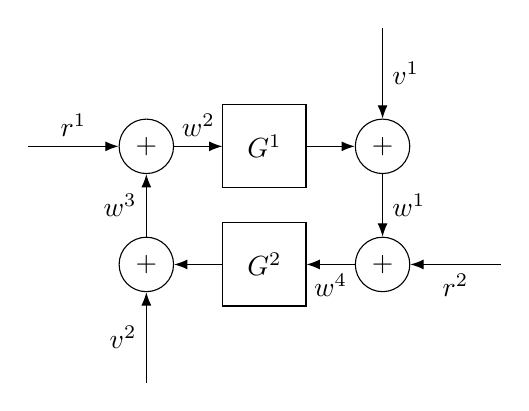
\begin{tikzpicture}[auto, node distance=2cm]

\node [input, name=r1] {};
\node [sum, right of=r1, node distance=1.5cm] (sum1) {$+$};
\node [block, right of=sum1, node distance=1.5cm] (G1) {$ G^1$};
\node [sum, right of=G1, node distance=1.5cm] (sum2) {$+$};
\node [input, above of=sum2, node distance=1.5cm] (v1) {};


\node [block, below of=G1, node distance=1.5cm] (G2) {$ G^2$};
\node [sum, below of=sum2, node distance=1.5cm] (sum3) {$+$};
\node [sum, below of=sum1, node distance=1.5cm] (sum4) {$+$};
\node [input, below of=sum4, node distance=1.5cm] (v2) {};
\node [input, right of=sum3, node distance=1.5cm] (r2) {};

% Draw edges
 \draw [-Latex] (r1) -- node {$ r^1$} (sum1);  
\draw [-Latex] (sum1) -- node {$ w^2$} (G1); 
\draw [-Latex] (G1) -- node {} (sum2);
\draw [-Latex] (v1) -- node {$ v^1$} (sum2);


 \draw [-Latex] (r2) -- node {$ r^2$} (sum3);  
\draw [-Latex] (sum3) -- node {$ w^4$} (G2); 
\draw [-Latex] (G2) -- node {} (sum4);
\draw [-Latex] (v2) -- node {$ v^2$} (sum4);

\draw [-Latex] (sum4) -- node {$ w^3$} (sum1);
\draw [-Latex] (sum2) -- node {$w^1$} (sum3);

 
\end{tikzpicture}}
\end{center}
\caption{Block diagram for a simple network.}
\centering
\label{fig:simple}
\end{figure}
%
The noise inputs $v^1_k,v^2_k$ and filtered external inputs
$r^1_k,r^2_k$ satisfy $v^1_k=H^1 e^1_k$, $v^2_k= H^2 e^2_k$ and
$r^1_k= Q^1 r_k$, $r^2_k= Q^2 r_k$. Assume that $H^1\not\equiv0$
and $H^2\not\equiv0$. The single input $r_k$ enters the loop at two nodes.
We are interested in estimating
$( G^1, Q^1)$, and use a predictor for
predicting $w^1_k$. We can measure $(w^3_k,r_k)$ in 
addition to $w^1_k$, and therefore the predictor input is $z_k=(w^1_k,w^3_k,r_k)$.
We obtain the 
following equations
%
\BEQ\label{eqn:example}
\begin{aligned}
\BBM w^1_k\\w^2_k\\w^3_k\\w^4_k\EBM&=
\BBM 0& G^1&0&0\\0&0&1&0\\0&0&0& G^2\\
1&0&0&0\EBM
\BBM w^1_k\\w^2_k\\w^3_k\\w^4_k\EBM+
\BBM 0&H^1&0\\ Q^1&0&0\\0&0&H^2\\Q^2&0&0\EBM \BBM r_k\\e^1_k\\e^2 _k\EBM\\
z_k&=\BBM 1&0&0&0\\0&0&1&0\\0&0&0&0\EBM
\BBM w^1_k\\w^2_k\\w^3_k\\w^4_k\EBM+\BBM 0\\0\\1\EBM r_k.
\end{aligned}
\EEQ
%
Here $\det P=1-G^1G^2$, so $P$ is generically invertible.
The graph contains three disjoint paths:
$(\mathcal U_2,\mathcal W_1,\mathcal Z_1)$,
$(\mathcal U_3,\mathcal W_3,\mathcal Z_2)$, and
$(\mathcal U_1,\mathcal Z_3)$. To check informativity for the fixed entries
in this example, we use the closed-loop transfer function matrix
%
$$\Pi =\BBM\frac{ G^1( Q^1+ G^2 Q^2)}{1- G^1 G^2}&\frac{H^1}{1- G^1 G^2}
&\frac{ G^1H^2}{1- G^1 G^2}\\
\frac{ G^2( G^1 Q^1+ Q^2)}{1- G^1 G^2}&\frac{ G^2H^1}{1- G^1 G^2}
&\frac{H^2}{1- G^1 G^2}\\
1& 0&0\EBM$$
%
which has determinant $H^1H^2/(1- G^1 G^2)$. Thus $\Pi$ has full row
rank when $P$ is well-posed and $H^1,H^2$ are nonzero transfer functions.
Under the predictor stability assumptions, a positive-definite spectrum for
$(r_k,e_k^1,e_k^2)$ at almost all frequencies therefore gives informativity.

The closed loop system transfer function from $(w^3_k,r_k)$ to $w^1_k$ is
given by
%
$$\setlength{\arraycolsep}{3.5pt}\BBM  G_c^1& G_c^2\EBM=\BBM 1&0\EBM\BBM 1&- G^1
\\0&1\EBM^{-1}\BBM 0&0\\1& Q^1\EBM
=\BBM  G^1& G^1Q^1\EBM.$$
%
The dimensions of the domain and the image closure are $\dim V_c=\dim V_o=2$ and we conclude that
%
$$( G^1, Q^1)=
( G_c^1, G_c^2/ G_c^1),\qquad G_c^1\not\equiv0.$$
%
Here, nonzero means not identically zero as a rational function.
Hence, we have generic network identifiability, and therefore also generic
local network identifiability. Uniqueness fails at $G_c=(0,0)$, where $G^1=0$
and $Q^1$ is arbitrary. This zero value is permitted by the structural pattern
but is nongeneric. Thus, identifiability does not hold for every admissible
closed loop transfer function.
%
\end{exmp}

\begin{exmp}
%
Let us now consider the case where we are only interested in estimating
$G^1$ and $Q^1$ is known. Using the same measured signals, we can form
$\xi_k=w_k^3+Q^1(q)r_k$. The network equation becomes
%
$$w_k^1=G^1(q)\xi_k+H^1(q)e_k^1.$$
%
Under the assumed innovation representation, let $V(q)$ be the predictor
transfer function from $\xi_k$ to $\hat w_k^1$. The predictor is
%
$$\hat w_k^1=W_y(q)w_k^1+V(q)\xi_k,\qquad G^1=(1-W_y)^{-1}V.$$
%
Equivalently, the original predictor columns are $(W_y,V,VQ^1)$. Following
Remark~\ref{rem:predictor-reduction}, it suffices to establish informativity of
$(w_k^1,\xi_k)$, rather than positive definiteness of the spectrum of all three
original predictor inputs.

With $e^2=0$, the transfer function matrix from $(r,e^1)$ to $(w^1,\xi)$ has determinant
%
$$-\frac{H^1(Q^1+G^2Q^2)}{1-G^1G^2}.$$
%
With $r=0$, the corresponding determinant for inputs $(e^1,e^2)$ is
%
$$\frac{H^1H^2}{1-G^1G^2}.$$
%
In either case, a positive-definite spectrum of the active inputs for almost all
frequencies ensures informativity when the displayed determinant is not
identically zero, under the standing well-posedness and stability assumptions.
Hence, known $Q^1$ allows reduced excitation by combining predictor inputs,
rather than simply discarding an unknown predictor column. This illustrates
how prior knowledge can reduce the excitation needed to identify $G^1$.
%
\end{exmp}

\begin{exmp}\label{ex:groebner-calculation}
%
Consider three unmeasured node signals $w_k=(w_k^1,w_k^2,w_k^3)$,
measured inputs $r_k=(r_k^1,r_k^2,r_k^3)$, and the measured output $y_k$.
Let $G$, $A$, and $H$ be unknown open-loop transfer functions, and take
%
\begin{align*}
P&=\BBM 1&-G&0\\0&1&0\\0&0&1\EBM, &
Q_r&=\BBM 1&0&0\\0&A&1\\0&A&0\EBM, &
Q_e&=\BBM 1\\0\\0\EBM,\\
R_y&=\BBM H&0&A\EBM, &
S_{yr}&=0, & S_{ye}&=0.
\end{align*}
%
Thus $w_k^2=Ar_k^2+r_k^3$, $w_k^1=Gw_k^2+r_k^1+e_k$,
$w_k^3=Ar_k^2$, and $y_k=Hw_k^1+Aw_k^3$. The same unknown $A$
occurs in two entries of $Q_r$ and one entry of $R_y$.
The closed-loop transfer function from $r_k$ to $y_k$ is
%
\begin{align*}
G_c&=R_yP^{-1}Q_r=\BBM H&HGA+A^2&HG\EBM\\
&=\BBM G_c^1&G_c^2&G_c^3\EBM.
\end{align*}
%
A generic fiber therefore satisfies
$H=G_c^1$, $G=G_c^3/G_c^1$, and
%
$$A^2+G_c^3A-G_c^2=0.$$
%
For $G_c^1\not\equiv0$ and $2A+G_c^3\not\equiv0$, this has exactly two
distinct solutions, $A$ and $A'=-G_c^3-A=-HG-A$. Both are rational transfer
functions and, when $G$, $H$, and $A$ are proper and stable, so is $A'$.
The Jacobian of $(G_c^1,G_c^2,G_c^3)$ with respect to $(G,A,H)$ has
determinant $-H(HG+2A)$, confirming generic local identifiability in the
algebraic sense. The quadratic shows that the generic fiber has two points,
so the network is not generically network identifiable. This fiber calculation
reveals the twofold ambiguity, which the generic Jacobian-rank test alone
does not distinguish from uniqueness.

For the predictor input $z_k=(y_k,r_k)$ and external signals
$u_k=(r_k,e_k)$, the determinant of the transfer function matrix $\Pi$ is $-H$.
Thus full generic row rank, and hence generic informativity under the
standing spectral and predictor assumptions, holds when $H\not\equiv0$.

The Gröbner basis rank test gives the same result. Here $\Pi$ is a
polynomial $4\times4$ matrix and $\det P=1$, so $D=1$. For $k=4$ its
ideal is $\mathcal I_4=\langle\det\Pi,1-t\rangle
=\langle H,1-t\rangle$. With $t$ first in the lexicographic order,
the reduced basis is $\{t-1,H\}$. Its polynomial independent of $t$
shows that rank falls below four exactly when $H=0$.

For the identifiability test, regard $G_c^1,G_c^2,G_c^3$ as output
variables over $K=\mathbb C(\lambda)$. The repeated unknown $A$ is a single
variable. The ideal defining the image closure is obtained by eliminating
$t,G,A,H$ from
%
$$\langle G_c^1-H,\ G_c^2-HGA-A^2,\ G_c^3-HG,\ 1-t\rangle.$$
%
For example, use lexicographic order
$t>G>A>H>G_c^3>G_c^2>G_c^1$. The resulting elimination ideal in
$K[G_c^1,G_c^2,G_c^3]$ is zero: when $G_c^1\neq0$, setting
$H=G_c^1$ and $G=G_c^3/G_c^1$ leaves the quadratic equation for $A$
above, which has a root over the algebraic closure of $K$.
Hence $\dim(V_c)=3=\dim(V_o)$, as required by the identifiability
criterion. The two roots give the generic twofold ambiguity.
%
\end{exmp}
%
\section{Computational Examples}
%
The following calculations use the Gröbner basis tests on a five-node
network. The MATLAB scripts and reproduction instructions are in the
accompanying supplementary archive \path{supplementary_matlab_code.zip}.
Its \path{README.md} identifies the two example scripts and three helper files.
For independent free entries, the path test avoids symbolic elimination.
A generic Jacobian-rank test decides whether fibers are finite; elimination
can additionally reveal the number of solutions and exceptional sets, as in
Example 3. Gröbner calculations can be costly as the number of unknowns
grows; the timings below describe these instances, not a scaling law.
%
\begin{exmp}
% Matlab sysid/file test_rational_dimension_cycle_5_c.m
Consider the dynamical network defined by $(P,Q_r,R_y,S_{yr})$, where $P=I-G$, $S_{yr}=0$ and 
%
\begin{align*}
G&=\BBM 0&G^{12}& 0 & 0 & 0\\
        0& 0& G^{23} & 0 &0\\
        0&0&0&G^{34}&0\\
        0&0&0&0&G^{45}\\
        G^{51}&0&0&0&0\EBM\\
Q_r&=\BBM Q^1&1&0&0&0\\
        0&Q^2&1&0&0\\
        0&0&Q^3&1&0\\
        0&0&0&Q^4&1\\
        Q^5&0&0&0&1\EBM\\
R_y&=\BBM R^1& 0 & 0& 0&0\\
        0& 1&0&0&0\\
        0&0&0&1&0\EBM.
\end{align*}
%
Here $\det P=1-G^{12}G^{23}G^{34}G^{45}G^{51}$, so $P$ is
generically invertible.
The eleven unknown open-loop transfer functions give $\dim V_o=11$. Elimination gives
$\dim V_c=11$, and hence generic local network identifiability in the
algebraic sense. With $Q_e=I$ and $S_{ye}=0$, the generic row rank of
$\Pi$ is eight, the number of predictor inputs; rank falls when $R^1=0$.
Theorem~\ref{thm:informativity} therefore gives generic informativity if the spectrum of
$(r_k,e_k)$ is positive definite for almost all frequencies and the
predictor is stable. The image-dimension computation took 631 seconds in
one run with MATLAB R2025a and Symbolic Math Toolbox 25.1 on an AMD Ryzen
7 250 with 31 GB RAM.
%
\end{exmp}
%
\begin{exmp}
In the same network, consider the subnetwork with unknown transfer
functions $(G^{12},Q^1,Q^2,R^1)$. Measure
$y_k=(R^1(q)w_k^1,w_k^2)$ and the boundary signal
$\tilde w_k^B=G^{23}w^3_k$. Its closed-loop transfer function is
%
$$F(X)=\BBM R^1&0\\0&1\EBM\BBM 1&-G^{12}\\0&1\EBM^{-1}\BBM 0&Q^1&1&0\\1&0&Q^2&1\EBM$$
%
for input $(\tilde w_k^B,r_k^1,r_k^2,r_k^3)$. The displayed $P_A$ has
determinant one. With $Q_e=I$ and
$S_{ye}=0$, the generic row ranks of $\Pi$ are eight, six, and five
when the active measured inputs are, respectively,
$(r_k^1,r_k^2,r_k^3,r_k^4,r_k^5)$, $(r_k^1,r_k^2,r_k^3)$, and
$(r_k^1,r_k^2)$.
In each case, a stable predictor and a positive-definite spectrum of the
active external signals for almost all frequencies give generic
informativity. The image dimension is four both for the displayed
$F(X)$ and after its last column is removed, so generic local network
identifiability also holds when $r_k^3=0$. The first and last columns
of $F(X)$ coincide.

\end{exmp}
%
\section{Conclusions}
%
Positive definiteness of the external-signal spectrum and full generic row
rank of the transfer function to the predictor inputs give a sufficient
condition for generic informativity. Vertex-disjoint paths determine that
rank for independent free entries; Gröbner bases also handle known or
constrained entries. The fiber-dimension test gives generic finite ambiguity
for the broader network model with unknown input and measurement transfer functions.
Example 3 has two admissible networks in a generic fiber, which the
Jacobian-rank test alone does not count. The algebraic genericity statements
do not certify a specified realization, and symbolic elimination can be
expensive even for small networks.
%
\section*{Acknowledgment}
OpenAI Codex was used to assist with drafting and revising text and proofs
in Sections I--IX, developing and checking the examples, and revising the
MATLAB code for the computational examples. The authors reviewed and edited
the resulting material and take responsibility for the article's content.
%
\section*{References}
\bibliographystyle{IEEEtran}        % Include this if you use bibtex 
\bibliography{refs}    
%
%\balance
%
\iffalse
\begin{IEEEbiography}[{
\includegraphics[width=1in,height=1.25in,clip,keepaspectratio]{victor_picture.jpeg}}]{João Victor Galvão da Mata} is a PhD candidate at the Technical University of Denmark (DTU). He received his B.S. degree in electrical engineering from the Federal University of Bahia (UFBA), Brazil, in 2021 and his M.S. degree from the University of Strasbourg, France, in 2022. His current research interests include optimization, numerical methods, linear systems, automatic control, system identification and dynamic networks. He was awarded the ``Grand Est Franco-German University Prize'' (Prix Universitaire Franco-Allemand Grand Est) in 2023 for the Best Master's Thesis in the category of Science and Technology.
\end{IEEEbiography}
%
\begin{IEEEbiography}[{
\includegraphics[width=1in,height=1.25in,clip,keepaspectratio]{anders_picture.jpg}}]{Anders Hansson} received the Master of Science degree in electrical engineering, the Degree of Licentiate of Engineering in automatic control, and the Ph.D. degree in automatic control from Lund University, Lund, Sweden, in 1989, 1991, and 1995, respectively. 
From 1995 to 1997, he was a Postdoctoral Student, and from 1997 to 1998, a Research Associate with Information Systems Lab, Department of Electrical Engineering, Stanford University, Stanford, CA, USA. In 1998, he was appointed  Assistant Professor and in 2000,  Associate Professor with S3-Automatic Control, Royal Institute of Technology, Stockholm, Sweden. In 2001, he was appointed Associate Professor with the Division of Automatic Control, Linköping University, Linköping, Sweden. Since 2006, he has been a Full Professor with the same department. He
was a Visiting Professor at the Department of Electrical and Computer Engineering, UCLA, Los Angeles, USA during 2011-2012. 
His research interests include optimal control, stochastic control, linear systems, signal processing, applications of control, and telecommunications. He is currently a Member of the EUCA General Assembly, of the Technical Committee on Systems with Uncertainty of the IEEE Control Systems Society and the Technical Committee on Robust
Control of IFAC.
\end{IEEEbiography}
%
\begin{IEEEbiography}[{
\includegraphics[width=1in,height=1.25in,clip,keepaspectratio]{martin_picture.jpeg}}]{Martin S.~Andersen} earned his MSc degree in Electrical Engineering from Aalborg University, Denmark, in 2006, and his PhD in Electrical Engineering from the University of California, Los Angeles (UCLA), USA, in 2011. Following his PhD, he served as a Postdoctoral Researcher at the Division of Automatic Control, Linköping University, Sweden, and the Technical University of Denmark (DTU). Currently, he is an Associate Professor in the Section for Scientific Computing, Department of Applied Mathematics and Computer Science at DTU. His research interests encompass optimization, numerical methods, signal and image processing, and systems and control.
\end{IEEEbiography}
\fi
%
\end{document}
